\section{Durchführung}
\label{sec:Durchführung}

\subsection{Einseitige Einspannung}
\label{sec:EinsetigeEinspannung}

\begin{figure} %[H]
    \centering
    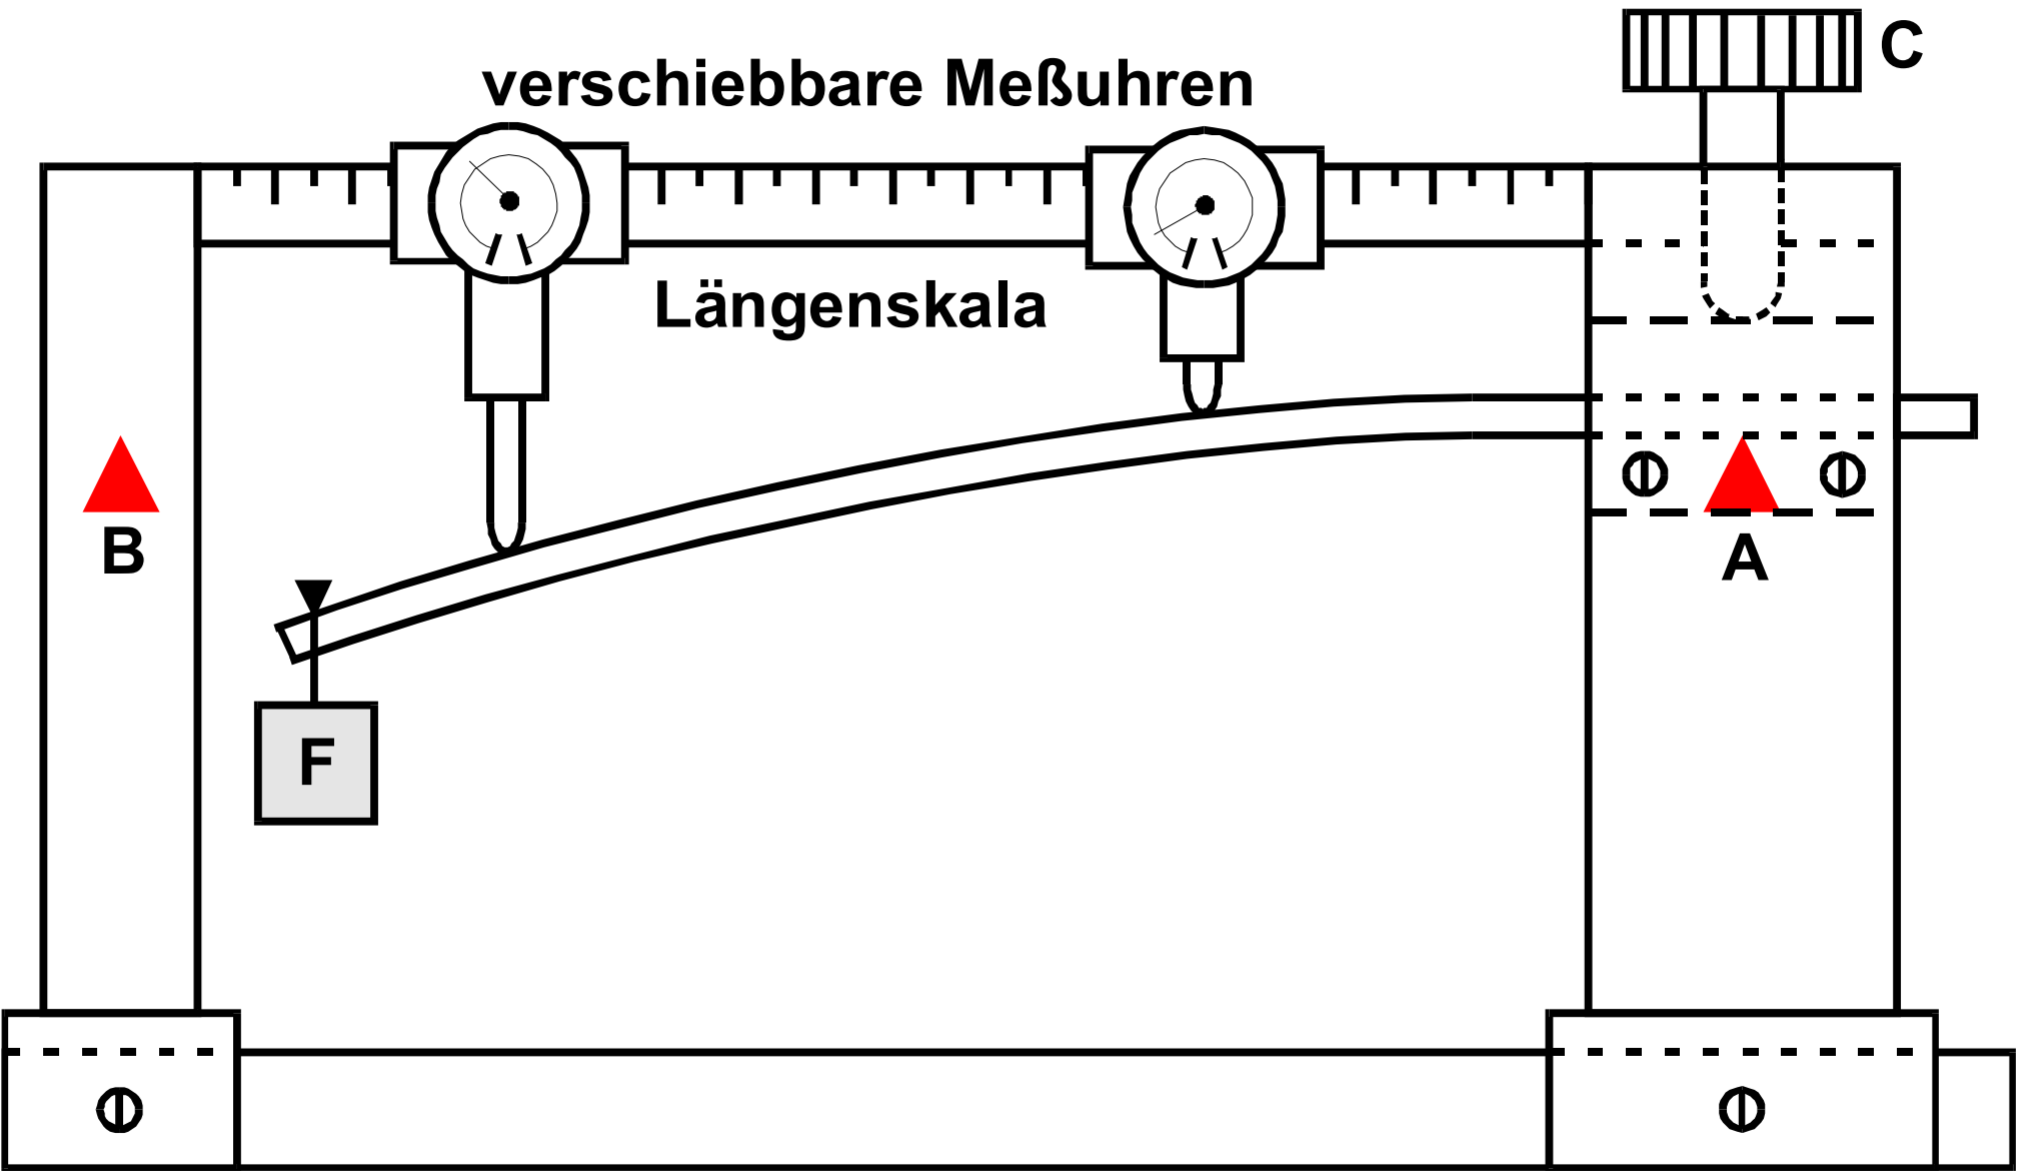
\includegraphics[width=\textwidth]{pictures/EinspannungEineSeite.png}
    \caption{Aufbau zur Messung elastischer Stäbe und deren Elastizitätsmodul \cite{v103}.}
    \label{fig:EinsetigeEinspannung}
\end{figure}

Um das Elastizitätsmodul $E$ eines Stabes zu bestimmen, wird zunächst der jeweilige Stab einseitig in die Apperatur
in Abbildung \ref{fig:EinsetigeEinspannung} am Fußpunkt A eingespannt.
Die Messung wird für einen eckigen Stab mit Länge $l_\text{eck} = 0.602 \unit\meter , m_\text{eck} = 0.5365 \unit{\kilo\gram}$
und der Seitenlänge $s = 0.01 \unit\meter$ durchgeführt.
Ebenfalls wird die Messung einen runden Stab mit den Eigenschaften $l_\text{run} = 0.59 \unit\meter , m_\text{run} = 0.4122 \unit{\kilo\gram}$
und einem Durchmesser von $d = 0.01 \unit\meter$ durchgeführt.
Um das Elastizitätsmodul $E$ richtig zu bestimmen, muss zunächst eine Nullmessung durchgeführt werden um die Messunsicherheit zu verringern.
Das bedeutet, es wird zunächst die Messuhr über den Stab geschoben und die Auslenkungen $D_0 (x)$ notiert.
Diese rechnet man hinterher heraus, um die vermeintlichen verbogenen Stellen des Stabes herauszurechnen, damit das Ergebnis nicht verfälscht wird.
Nun wird ein Gewicht von $m = 0.654 \unit{\kilo\gram}$ an den Stab herangehängt.
Dabei ist das Gewicht so nah am Ende des Stabes, als dass es als nahtlos am Ende angehängt angenommen werden kann.
Nun wird die Messuhr erneut über den Stab geschoben und die Auslenkungen $D_m (x)$ werden ebenfalls notiert.

\subsection{Beidseitige Einspannung}
\label{sec:BeidseitigeEinspannung}

Es wird die selbe Konstruktion wie in Abbildung \ref{fig:EinsetigeEinspannung} benutzt, mit der Ausnahme, dass nun beide Seiten aufgelegt werden.
Das bedeutet, das \enquote{herabhängende} Ende wird nun auf den Fußpunkt B gelegt.
Im Unterschied zur einseitigen Messung, werden in diesem Aufbau zwei verschiedene Uhren genommen.
Das bedeutet auch, das für jeweils beide eine Nullmessung vorgenommen werden muss.
Dann werden wieder die Auslenkungen $D_0 (x) \text{ und } D_m (x)$ gemessen.
Bei der Messung für $D_m (x)$ wird ein Gewicht von $m = 1.5524 \unit{\kilo\gram}$ in die Mitte gehängt.
Diese Messung wird jeweils für den eckigen und runden Stab vorgenommen.
Außerdem kann aufgrund der beiden Messuhren, nur bis zur Mitte des Stabes gemessen werden.